\section{Theory and experimental setup}
\subsection{Metal-semiconductor junctions}
Consider a metal and an $n$-type semiconductor separated from each other, as depicted on the left of \autoref{fig:schottky_barrier}.
\begin{figure}[htbp]
    \centering
    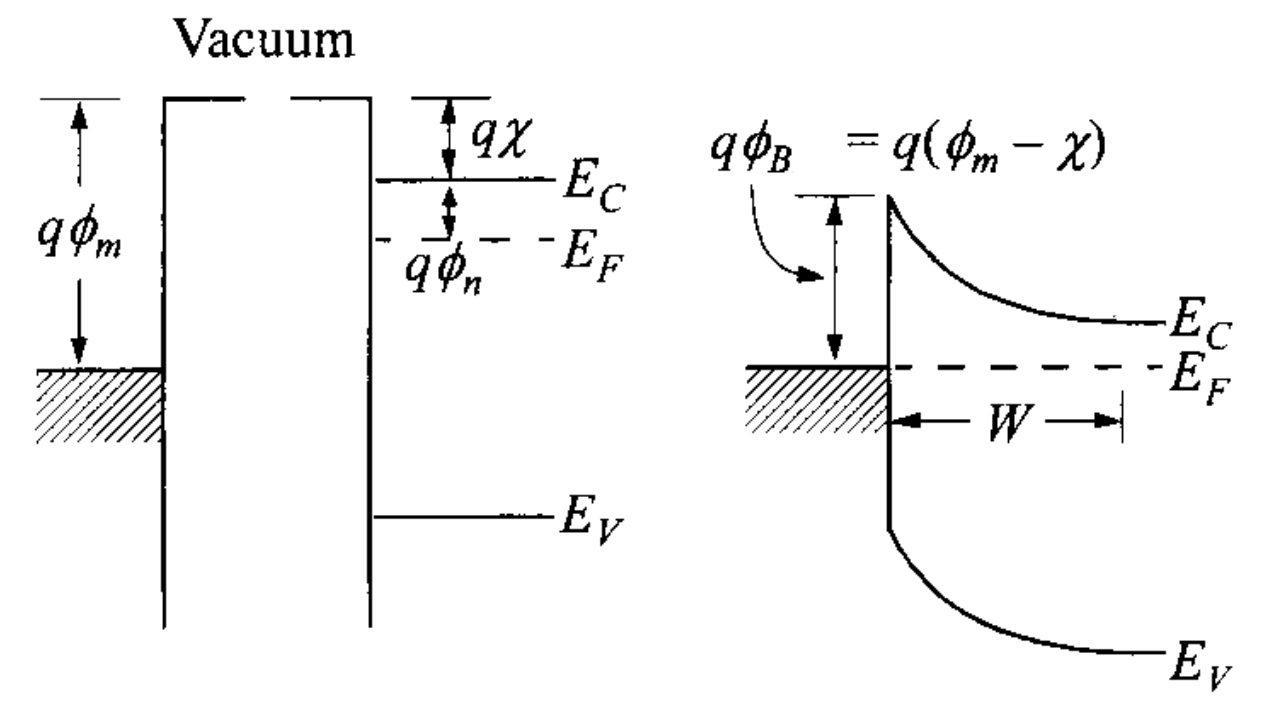
\includegraphics[width=12cm]{figures/schottky_barrier.png}
    \caption{}
    \label{fig:schottky_barrier}
\end{figure}
Their work function, defined as the energy difference between the vacuum level and the Fermi level $E_F$, is equal to $q \phi_m$ for the metal ($q$ is the charge of \hl{the electron?}) and to $q (\chi + \phi_n)$ for the semiconductor, where $q \chi$ is the electron affinity measured from the bottom of the conduction band $E_c$ to the vacuum and $q\phi_n$ is the energy difference between $E_c$ and $E_F$ \cite{sze_physics_2007}.
When the two materials are put in contact, electrons flow from the semiconductor\hl{, where the mean energy is greatest,} to the metal until their Fermi levels line up.
A negative charge is accumulated in the metal, and a correponding positive one in the semiconductor, causing the formation of an internal electric field and of a potential barrier known as \emph{Schottky barrier}.
For an ideal metal-semiconductor contact, its height $\phi_b$ is the difference between the metal work function and the electron affinity of the semiconductor \cite{sze_physics_2007}:
\begin{equation} \label{eq:barrier_height}
    q\phi_b = q(\phi_m - \chi)
\end{equation}

Though we neglect surface-state effects, \autoref{eq:barrier_height} is generally valid \cite{sze_physics_2007}:
Even if the contact is not perfect and a very thin interfacial layer separating metal and semiconductor still remains, this layer is usually so thin ($\sim 10$ \AA) that electrons can easily pass through it by tunnelling \cite{rhoderick_physics_1970}.
More complex models must be applied when the layer is known to be larger.

This barrier gives the junction rectifying properties, as it must be surmounted for the electrons to flow from the metal into the semiconductor.
This behaviour is the basis of an array of electronic components, like Schottky diodes and transistors.
\hl{Advantages of schottky diodes?}

\subsection{Measurement of barrier height}
\hl{Alternativement une sous-section pour chaque méthode}
In this work the Schottky barrier of a Au-Si \hl{??} MS was determined using two different methods:


\paragraph{Current-Tension curves}
\emph{explain/present Thermionic-Emission Theory}
\begin{equation} \label{eq:IV-curve}
    V = \frac{n k_N T}{q} \ln \left( \frac{I}{I_S} +1 \right) + RI
\end{equation}
For electrons ($n$-type Si), $A^{**}$ in the field range $10^4$ to $2\times 10^5$ V/cm remains essentially at a constant value of about 110 \unit{A cm^{-2} K^2}.

A $100 \%$ increase in $A^{**}$ will cause an increase of only $0.018$ V in $\phi_b$.

The principal mechanism responsible for the current flow at the majority of Schottky diodes on non-degenerate semiconductors has been shown by various studies to be the thermionic emission process \cite{tung_recent_2001}.

Even though $n$ is known as the  "ideality" factor, its numerical value actually reflects the departure from ideality; namely, the larger $n$ is, the less "ideal" is said of the SB \cite{tung_recent_2001}.
Generally speaking, the ideality factor is an indicator of the bias dependence of the SBH. With increasing forward bias, there is a tendency for the effective SBH which controls the current transport to also increase, giving rise to $n > 1$.

\paragraph{Photoelectric measurement}


\subsection{Setup for I-V measures}
The sample, a Au-Si junction, was put in a cryostat to lower and control its temperature.
Measures were conducted between $124 \pm ?$ and $296\pm?$ K. 
A function generator sweeped the applied voltage at a frequency of $??$ Hz between $0$ and $2.5$ V while an amperemeter measured the current.

The curves were fit using \autoref{eq:IV-curve} to obtain parameters blablabla.
Then $\phi_b$.
